\section{\papername Tensorization and Compression} \label{sec:formulation}

\begin{figure*}[t]
\centerline{
\includegraphics[width=1\textwidth]{figures/formulation.pdf}}
\vspace{-0.2cm}
\caption{Formulating the (a) maximum likelihood decoding as (b) minimizing the free energy of the spin glass model, and using (c) the tensor network to calculate the free energy.} 
\vspace{-0.4cm}
\label{fig:formulation}
\end{figure*}

To balance the decoding accuracy and computational complexity, we first convert the constrained calculation into an unconstrained summation format. Then, the computation for this summation is tensorized using the spin glass model, where 
the errors and syndromes are converted into spins. After this, the logical probabilities are calculated by the free energies of the spin glass system, which can be efficiently computed by the tensor network.
Although the tensorization exposes the opportunity to parallel the MLD computation, the overall memory footprint and computational workload (FLOPs) still grow exponentially with the qLDPC code size. Identifying that the tensors from the spin glass model can be expressed by a product of constant-dimensional matrices, we propose an exact tensor decomposition that shrinks the original $O(2^n)$ tensor to a matrix product state (MPS) with a linear complexity of $O(8n)$, from 
3.9GB to 8.7KB for 254-size trivariate bicycle codes. To further reduce the computational workload, we flatten the high-dimensional connection in MPS into a 1D chain. We achieve this by swapping the tensor indices and merging adjacent matrices to eliminate high-dimensional connections without loss of logical probability information. Finally, we successfully compress the computation requirement from 6.1 TFLOPS to 48 KFLOPS, with little accuracy loss.



\subsection{Tensorizing MLD with Spin Glass Model}

Calculating the logical error probability with \eqref{eq:logicalprobcons} is non-trivial, as we need to determine the total probability by scanning all physical errors that satisfy two constraints: 1) belong to the same logical error.  2) produce the observed syndrome;
Since checking these two constraints will consume computing resources, we tend to convert the formula into an unconstrained summation format. Clearly, as shown in \autoref{fig:formulation}~(a), we decompose the logical error space $\vec{e}_Z$ into stabilizer subspaces $H_Z^T$ that are shifted by destabilizers $H_{\text{des}}^T$ and logical operators $L_Z^T$,
\begin{equation}\small
    \vec{e}_Z= H_Z^T \vec{z} \oplus H_{des}^T\vec{s}\oplus L_Z^T\vec{l},\forall \vec{z}\in\{0,1\}^M
\end{equation}
Combining this equation with the logical probability $P(\vec{l}|\vec{s})$ in \eqref{eq:logicalprobcons} gives an unconstrained summation over all possible stabilizers $\vec{z}$ as
\begin{equation}\label{eq:logicalstabsummation}
    P(\vec{l}|\vec{s}) =  \textstyle  \sum_{\vec{z} \in \{0,1\}^M} P(H_{\text{des}}^T \vec{s} \oplus H_Z^T \vec{z} \oplus L_Z^T \vec{l})\;.
\end{equation}
The mathematical derivation is summarized in \hyperref[subsec:proofA]{Appendix A}.

However, this summation still has exponential complexity.
To further simplify this, we recast the decoding problem within the framework of the spin glass model, which has broad application in discrete optimization problems~\cite{wiki_spin_glass}. A representative application is that this model is widely used in statistical mechanics to study systems with disorder and frustrated interactions, matching the properties of our formulation. Concretely, the error in decoding problem has two discrete states, 0 or 1, which resemble the two states in the spin glass model, the up(+1) and down(-1) spin rotations. This inspires us to represent stabilizer bits $\vec{z}$, syndrome $\vec{s}$, and logical bits $\vec{l}$ in ~\eqref{eq:logicalstabsummation} as stabilizer spins $\vec{t}$, syndrome spins $\vec{y}$ and logical spins $\vec{g}$ via the bits-to-spin mapping,
\begin{equation}
    (-1)^{z_k} = t_k, ~~(-1)^{s_k} = y_k, ~~(-1)^{l_k} = g_k\;.
\end{equation}
As shown in \autoref{fig:formulation}~(b), mapping bits to spins transforms the probability into the energy of a spin glass determined by the Hamiltonian $H$,
\begin{equation}\small
    H = -\sum_{j=1}^{n} \omega_j\prod_{\{k|H_z(k,j)\neq0\}} t_k  \prod_{\{k|H_{\text{des}}(k,j)\neq0\}} y_k  \prod_{\{k|L_z(k,j)\neq0\}} g_k \;.
\end{equation}
 The logical error probability under the spin glass system is
\begin{equation}\small\label{eq:logicalprobfreeenergy}
    P(\vec{l}|\vec{s})=  \textstyle \sum_{\vec{t}\in\{-1,1\}^{M}} e^{-H}
\end{equation}
The mathematical derivation is summarized in \hyperref[subsec:proofB]{Appendix B}. 

% This equation is related to the free energy $F$ of the spin glass model in statistical mechanics by $F = -\ln P(\vec{l}|\vec{s}) $~\cite{chubb2021statistical}. 
Finally, it has been demonstrated that the spin glass model can be efficiently calculated via a tensor network~\cite{cao2025exact}, exposing the opportunity to tensorize \eqref{eq:logicalprobfreeenergy}. By mapping the energy terms and spin variables in \autoref{fig:formulation}~(b) to the energy tensor $T_j$ and Kronecker Tensor $\delta$, we convert the summation operation in \eqref{eq:logicalprobfreeenergy} into the contraction of the tensor network $\mathcal{T}$ in \autoref{fig:formulation}~(c). As a result, the logical error probability $P(\vec{l}|\vec{s})$ is reformulated as the contraction of the tensor network $\mathcal{T}$. Here is the formal lemma, where the proof can be found in \hyperref[subsec:proofC]{Appendix C}.
\begin{lemma}\label{theorem:decodingTensor}
    The probability of logical error $\vec{l}$ with given syndrome $\vec{s}$, noted as $P(\vec{l}|\vec{s})$, can be calculated via tensor network $\mathcal{T}$ contraction as
    \begin{equation}\small
    P(\vec{l}|\vec{s}) = 
    \frac{{\text{contract}}(\mathcal{T}(\vec{l},\vec{s}))}{\text{contract}(\mathcal{T}(\vec{s}))}. 
    \end{equation}
\end{lemma}

% Since the spin glass model can be efficiently calculated via a tensor network~\cite{cao2025exact}, we thus try to convert \eqref{eq:logicalprobfreeenergy} into tensor computations.
% Through mapping the energy terms and spin variables in \autoref{fig:formulation}~(b) to the energy tensor $T_j$ and Kronecker Tensor $\delta$, we convert the summation operation in \eqref{eq:logicalprobfreeenergy} into the contraction of the tensor network $\mathcal{T}$ in \autoref{fig:formulation}~(c).
% % Typically, the free energy of the spin glass model can be efficiently computed with contraction on the tensor network $\mathcal{T}$ in \autoref{fig:formulation}~(c)~\cite{cao2025exact,chubb2021statistical}.
% Finally, the logical error probability $P(\vec{l}|\vec{s})$ is calculated with the contraction of the tensor network $\mathcal{T}$, as formally stated in the following lemma.


This tensor network $\mathcal{T}$ contains energy tensor $T_j$ and Kronecker tensor $\delta_i$, which are defined as
\begin{equation} \label{eq:tensorT}\small
    T_j[\alpha_1][\alpha_2]\cdots= \exp \left(\omega_j \prod_{k} (-1)^{\alpha_k}\right)
\end{equation}
\begin{equation}\small
    \delta_i[\alpha_1][\alpha_2]\cdots = \begin{cases}
        1,\text{if}\;\alpha_1 =\alpha_2 = \cdots \\
        0, \text{else}
    \end{cases}\label{eq:tensordelta}
\end{equation}
where $\omega_j$ is the error weight of the $j$-th physical error, which is calculated from physical error rate $p_j$ by \eqref{eq:errorrate}. $\alpha_k$ is the indices of each tensor which has two value $\{0,1\}$. Furthermore, the \eqref{eq:tensorT} can be rewritten as the expression of $p_j$,
\begin{equation} \label{eq:tensorTcases}\small
    T_j[\alpha_1][\alpha_2]\cdots= \begin{cases}
        \sqrt{p_j/(1-p_j)},\text{if}\; \sum_{k} \alpha_k = 1\;\text{mod 2}\\
        \sqrt{(1-p_j)/p_j}, \text{if}\; \sum_{k} \alpha_k = 0\; \text{mod 2}
    \end{cases}
\end{equation}
\autoref{fig:tensor_example} plots a numerical example of these two types of tensors, which are derived from the 18-size BB code under physical error rate $p_j=0.1$. For instance, here are two tensor elements.
\begin{equation} \small
\begin{aligned}
    & T_j[0][1][1][0][1][0]= 0.1, \\
    & T_j[1][1][1][0][1][0]= 10 \notag    
\end{aligned}
\end{equation}
For the six-rank Kronecker tensor $\delta_j$, only two elements are one and the rest are zeros.
\begin{equation} \small
\begin{aligned}
    & \delta_j[0][0][0][0][0][0]= 1, \\
    & \delta_j[1][1][1][1][1][1]= 1 \notag    
\end{aligned}
\end{equation}

% These tensors are linked as the Tanner graph, and each connected edge is the indices to be contracted, as shown in the tensor network $\mathcal{T}$ of \autoref{fig:formulation}~(c). 

\begin{figure}[t]
\centerline{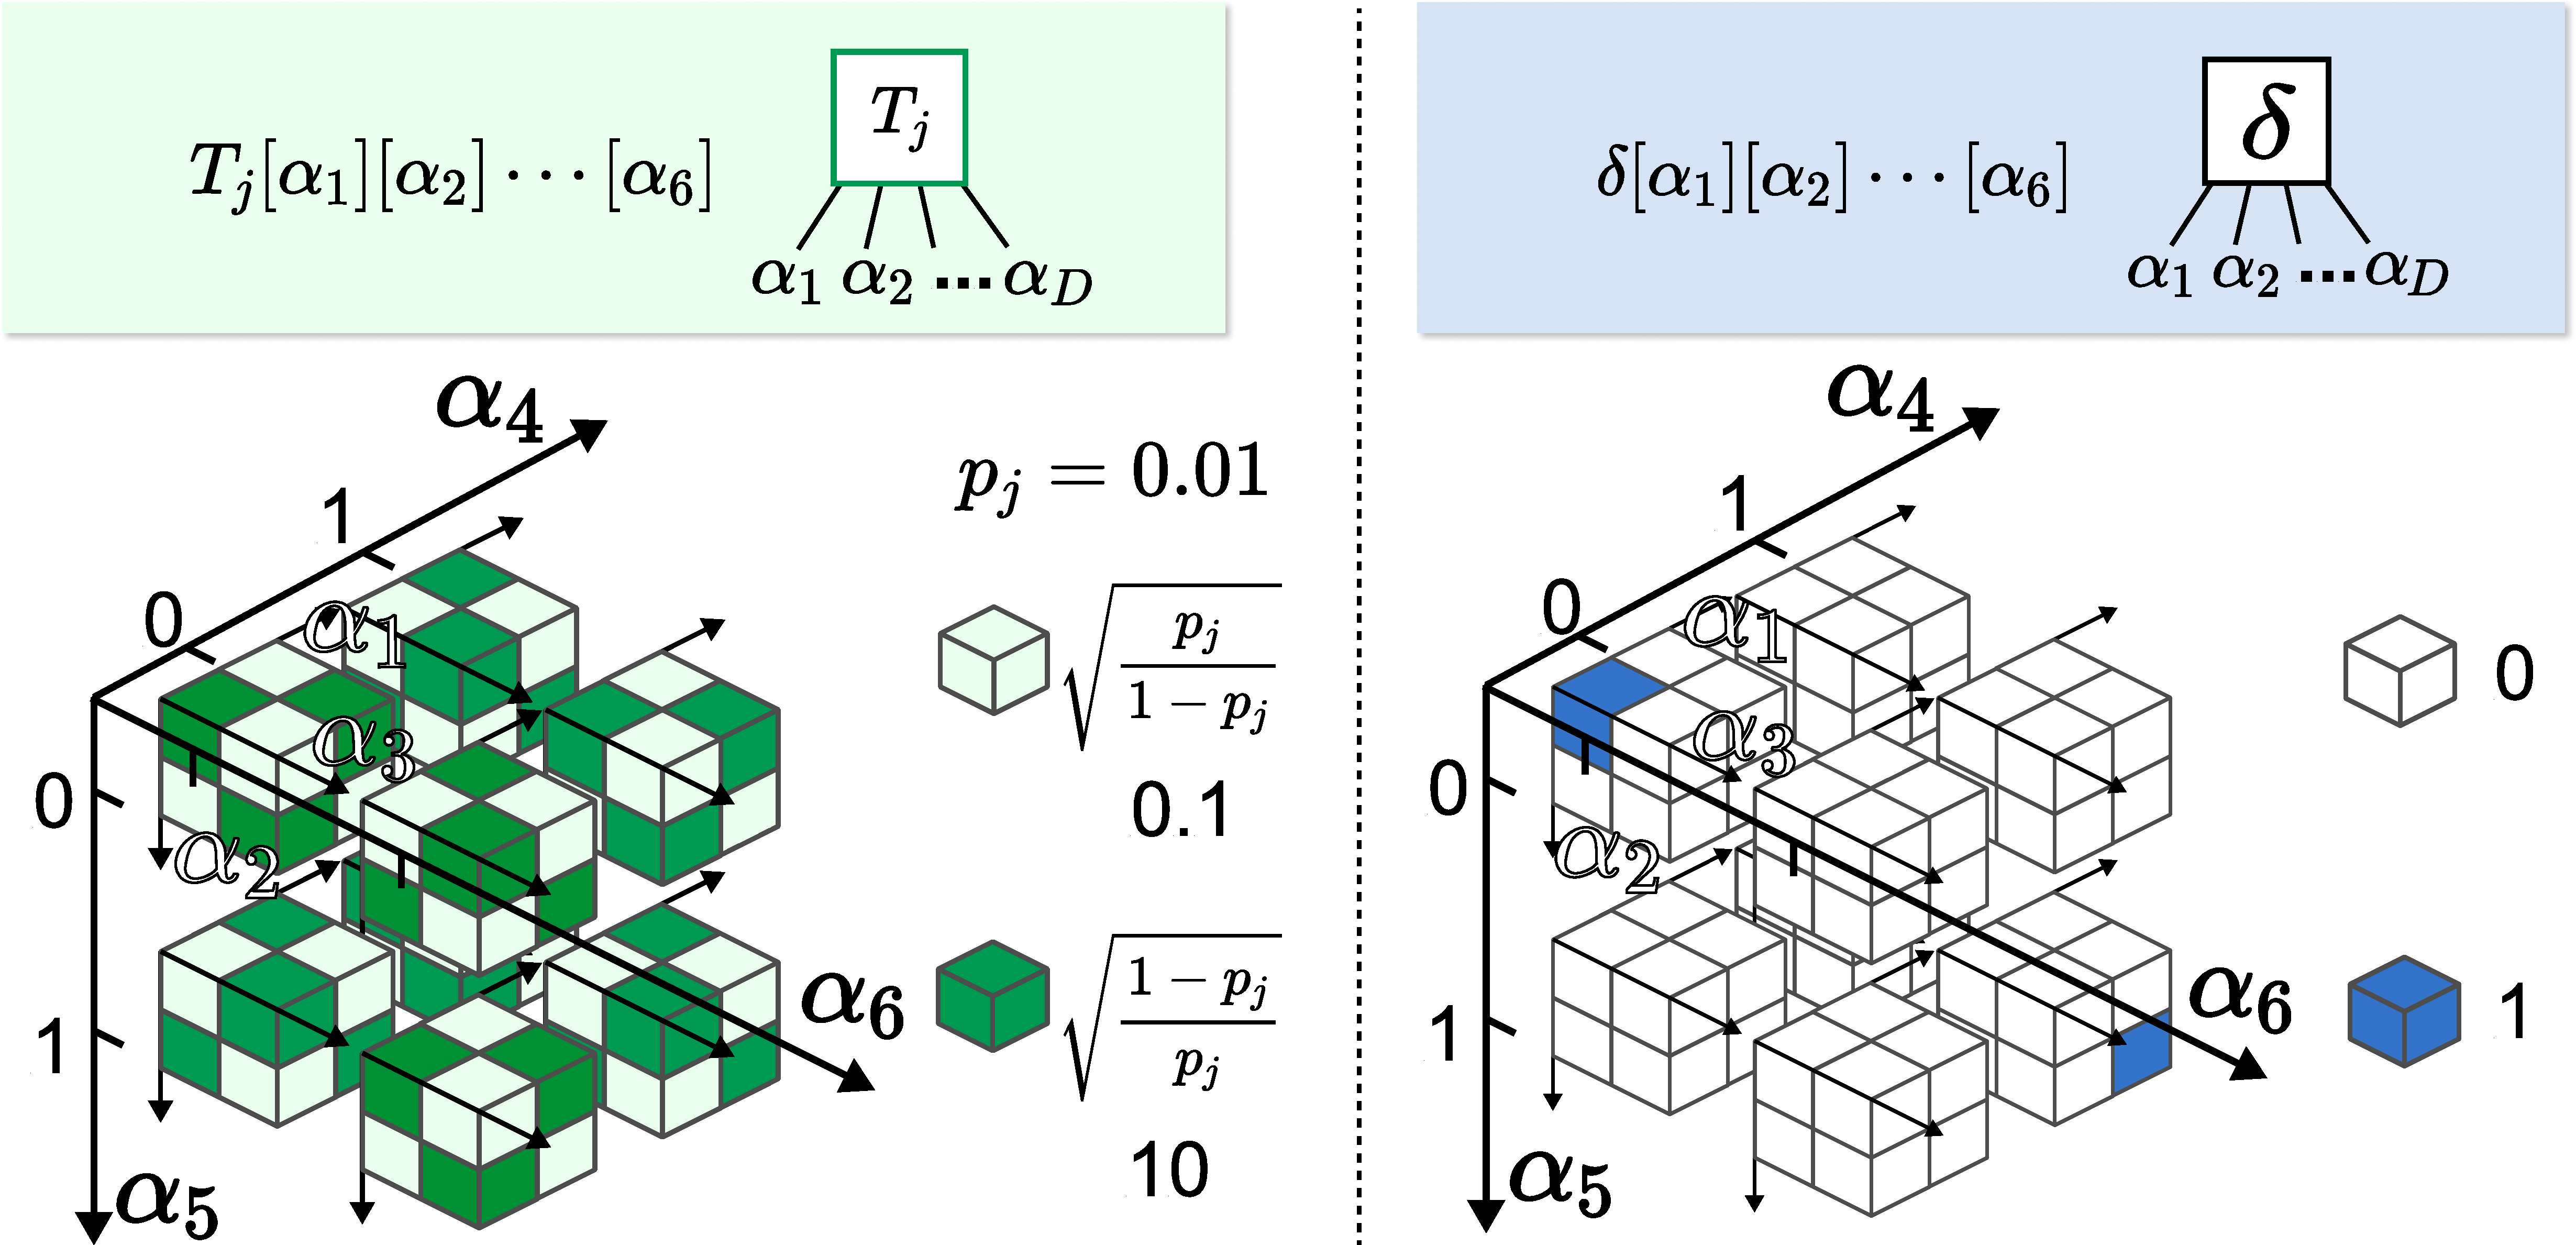
\includegraphics[width=1\columnwidth]{figures/TensorExample.pdf}}
\vspace{-0.3cm}
\caption{The numerical example of the tensors used in the tensor network decoder.} 
\label{fig:tensor_example}
\end{figure}

\subsection{Exact Tensor Decomposition via Matrix Product State}

The raw tensor network involves n-rank tensors with $2^n$ elements, leading to huge computation cost and memory bottleneck. Prior compression techniques often employ singular value decomposition to decompose the tensors into low-rank matrix product states (MPS) or tree tensor network states~\cite{pan2020contracting,ma2024approximate}. However, this coarse-grained decomposition only saves the top largest singular values of tensors and drops the other singular values, causing a significant accuracy loss.

% The tensors in the original tensor network, as shown in \autoref{fig:formulation}~(c), are high-rank tensors with $2^n$ elements, making the contraction suffer from high computation cost and memory bottleneck. Prior work on tensor network contraction using singular value decomposition to decompose the tensors into low-rank Matrix Product States (MPS) or tree tensor network states~\cite{pan2020contracting,ma2024approximate}. \hl{This decomposition only saves the top largest singular values of tensors and drops the other singular values, causing an accuracy loss. }
% \hl{why there is a great accuracy loss?}



\begin{figure}[t]
\centerline{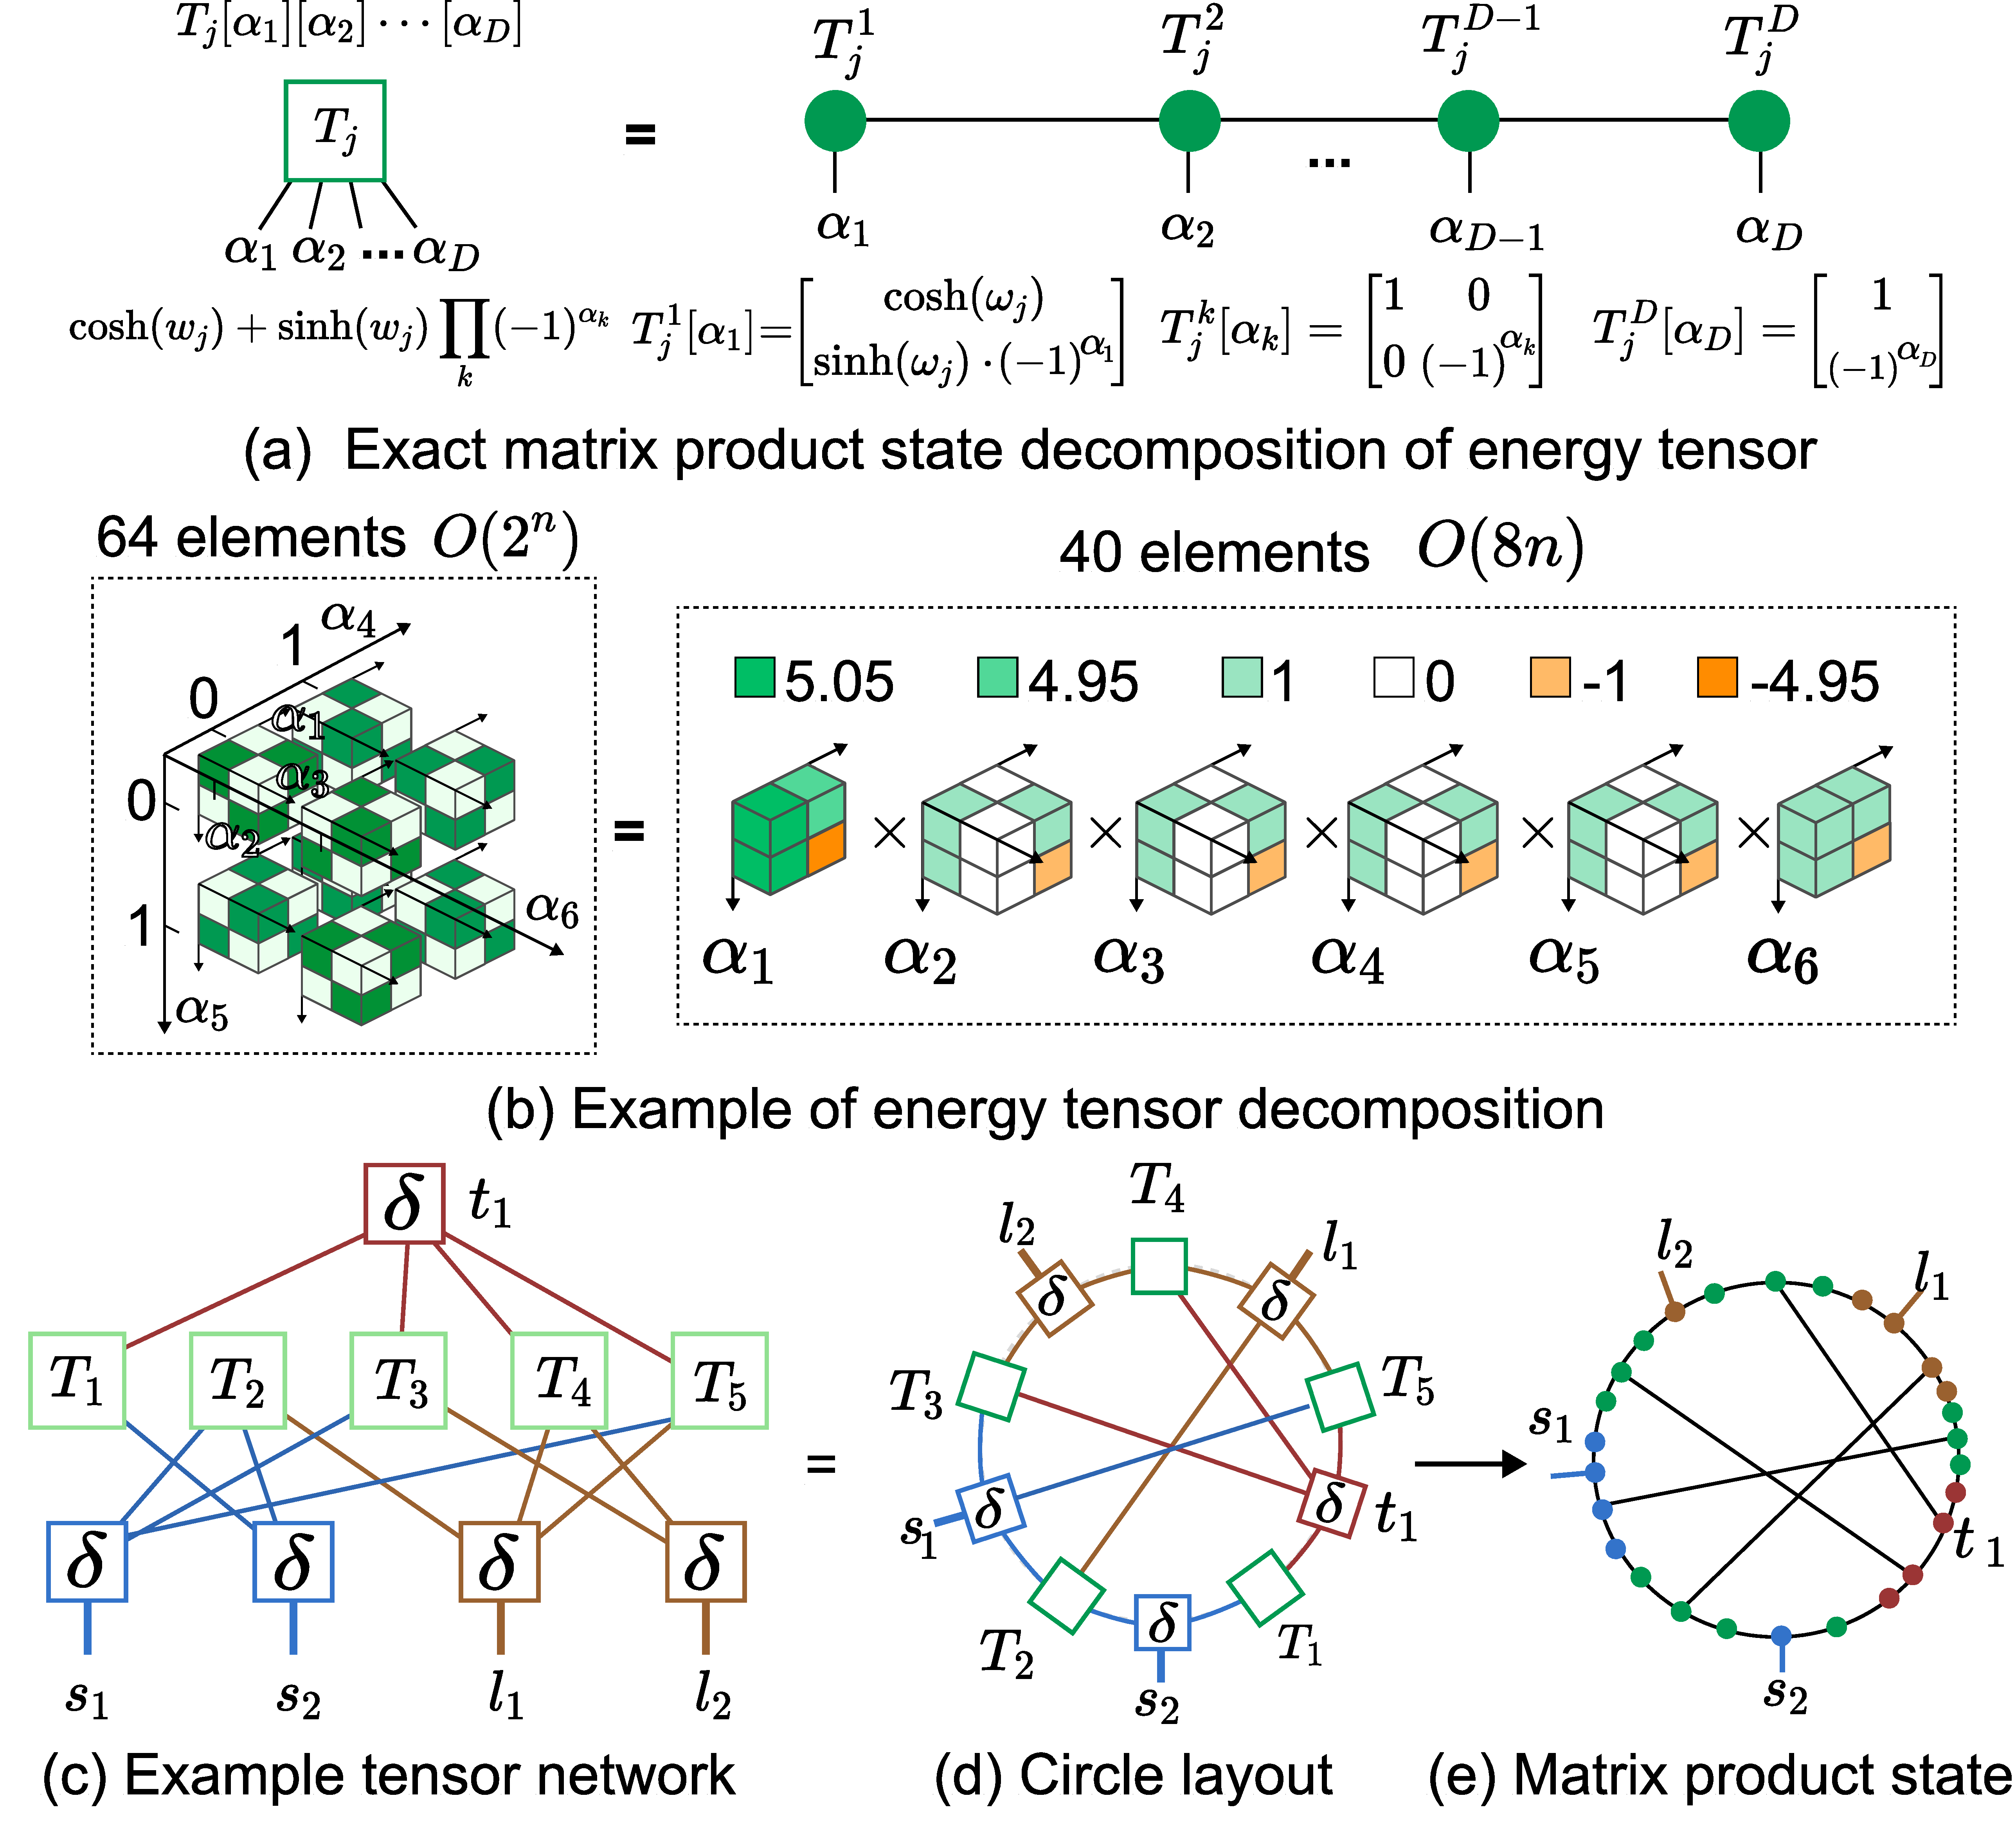
\includegraphics[width=1\columnwidth]{figures/mps.pdf}}
\vspace{-0.3cm}
\caption{Decomposing the tensor network into matrix product states.} 
\vspace{-0.2cm}
\label{fig:mps}
\end{figure}

%先讲讲我们的考虑，我们是怎么想到exact decomposition，为什么我们可以exact，再给具体数学细节
% \hl{insight, motivation, how we got this?}
Considering the binary nature of the errors and check matrices in MLD, we observe that the tensors derived from the spin glass model exhibit a highly structured nature. The pattern includes: 1) each element only has two values (\eqref{eq:tensordelta} and \eqref{eq:tensorTcases}); 2) the same values are in diagonal distribution or interleaved distribution. Identifying these features, we propose an exact decomposition scheme that can equivalently decompose the tensor into a series of smaller matrices, as
shown in \autoref{fig:mps}~(a). 
Specifically, since the results of spin multiplication only have two values, -1 or 1, the tensor can only be $e^{-\omega_j}$ and $e^{\omega_j}$, transforming the tensor $T_j$ in \eqref{eq:tensorT} to hyperbolic functions.
\begin{equation} \small
    T_j = \cosh (\omega_j) + \sinh (\omega_j) \prod_k (-1)^{\alpha_k}
\end{equation}
We can verify that this tensor $T_j$ can be represented by matrix products with the tensors $T_j^k$ in \autoref{fig:mps}~(a).
\begin{equation}\small
    T_j[\alpha_1][\alpha_2]\cdots[\alpha_D] = \prod_{k=1}^{D} T^k_j[\alpha_k]
\end{equation}
\autoref{fig:mps}~(b) gives the example of decomposing a six-rank energy tensor into six three-rank tensors, shrinking the tensor size from 64 elements to 40 elements.
For the tensor $\delta$ in \eqref{eq:tensordelta}, the elements that share the same index $\alpha_k$ have the same values. Thus, it can be exactly decomposed into low-rank tensors $\delta$.
\begin{equation}\small
    \delta[\alpha_1]\cdots[\alpha_D] = \sum_{\vec{\beta}} \delta[\alpha_1][\beta_1] \delta[\beta_1] [\alpha_2] [\beta_2]\cdots \delta[\beta_{D-1}] [\alpha_D].
\end{equation}

\autoref{fig:mps}~(c)-(e) visualizes the tensorization process of the entire tensor network, where the tensor network is derived from \autoref{fig:formulation}~(c). To better understand dimension reduction, \autoref{fig:mps}~(d) organizes it in a circular layout, maintaining the original connectivity. In this circle, we can observe that each tensor is connected with four neighboring tensors at most. By decomposing it into matrix product states, the tensors are converted into three-rank tensors or two-rank tensors, and each has at most three neighbors, as depicted in \autoref{fig:mps}~(e).

% Using the exact matrix product state decomposition, we can represent the original high-rank tensors into two-rank tensors or three-rank tensors, reducing the memory complexity from $O(2^n)$ to $O(8n)$. For instance, the tensor network in \autoref{fig:mps}~(b) contains ten tensors with four-rank at most. If we organize it in a circle layout as shown in \autoref{fig:mps}~(c), we can see that the tensors in the graph show a high-dimensional connection with four neighboring tensors at most. By decomposing it into matrix product states, the tensors are converted into three-rank tensors or two-rank tensors, and each has at most three neighbors, as depicted in \autoref{fig:mps}~(d).






\subsection{Tensor Network Compression by Offline Contraction}

Although MPS partially addresses the computational pressure, especially the memory bottleneck, there remain tremendous computations arising from the high-dimensional connections among matrices. A natural idea is to compress the connectivity offline and introduce a low-dimensional topology MPS when online decoding. Observing that the high-dimensional connection basically results from the internal edges in the circle, as shown in \autoref{fig:mps}~(d), our intuition is to eliminate these internal edges. To achieve this goal, we propose the \textit{contraction-swap-merge} method, which iteratively contracts the small tensors, swaps the tensor indices to put the internal edges in adjacent positions, and merges these edges. These three operations used in this method are defined as follows.
% \hl{three operator.}
\begin{itemize}
    \item The \textit{contract} operation is the basic operation in the tensor network, which merges two adjacent tensors into a new tensor by contracting the edge index between them, as shown in \autoref{fig:operations}~(a). The cost of \textit{contract} operations between two tensors with $d_1$ dimensions and  $d_3$ dimensions is $O(d_1d_2d_3)$, where $d_2$ is the bond dimension between them (The bond dimension is the dimension of the multiplication between two tensors). 
    
    \item The \textit{swap} operation is defined as swapping the two adjacent indices in MPS, such as the $\alpha_2$ and $\alpha_3$ indices in \autoref{fig:operations}~(b). The \textit{swap} cost differs in two cases. Swapping between pairs like $(T,T)$, $(T,\delta)$,$(\delta,\delta)$ has no cost. However, for other cases, swapping between tensors needs to use a contract operation and singular value decomposition with cost $O(d^6)$. This will introduce accuracy loss due to the singular value decomposition is an approximated Ddecomposition~\cite{ma2024approximate}. 
    
    \item The \textit{merge} operation uses two contract operations to merge the adjacent edges between two MPS into one edge with a higher dimension. The cost of the \textit{merge} operation comes from the \textit{contract} operation, as shown in \autoref{fig:operations}~(c).
\end{itemize}


% Matrix product state (MPS) solves the memory bottleneck caused by high-rank tensors but still suffers from the high contraction cost due to the high-dimensional connections between matrix product states, making the deployment on a real-time hardware decoder impractical. A natural idea is to reduce the dimension of the connection topology offline and use a low-dimensional topology matrix product state for online decoding. We further identify that the high-dimensional connection is due to the additional connection edges between each tensor, such as the edges inside the circle in \autoref{fig:mps}~(c). Our intuition is to eliminate these entanglement edges and obtain a tensor network with only tensors on the circle, which is exactly a 1D-chain matrix product state that can be efficiently stored and contracted. To execute this strategy, we designed a \textit{swap-merge-contraction} method. 


\begin{figure}[t]
\centerline{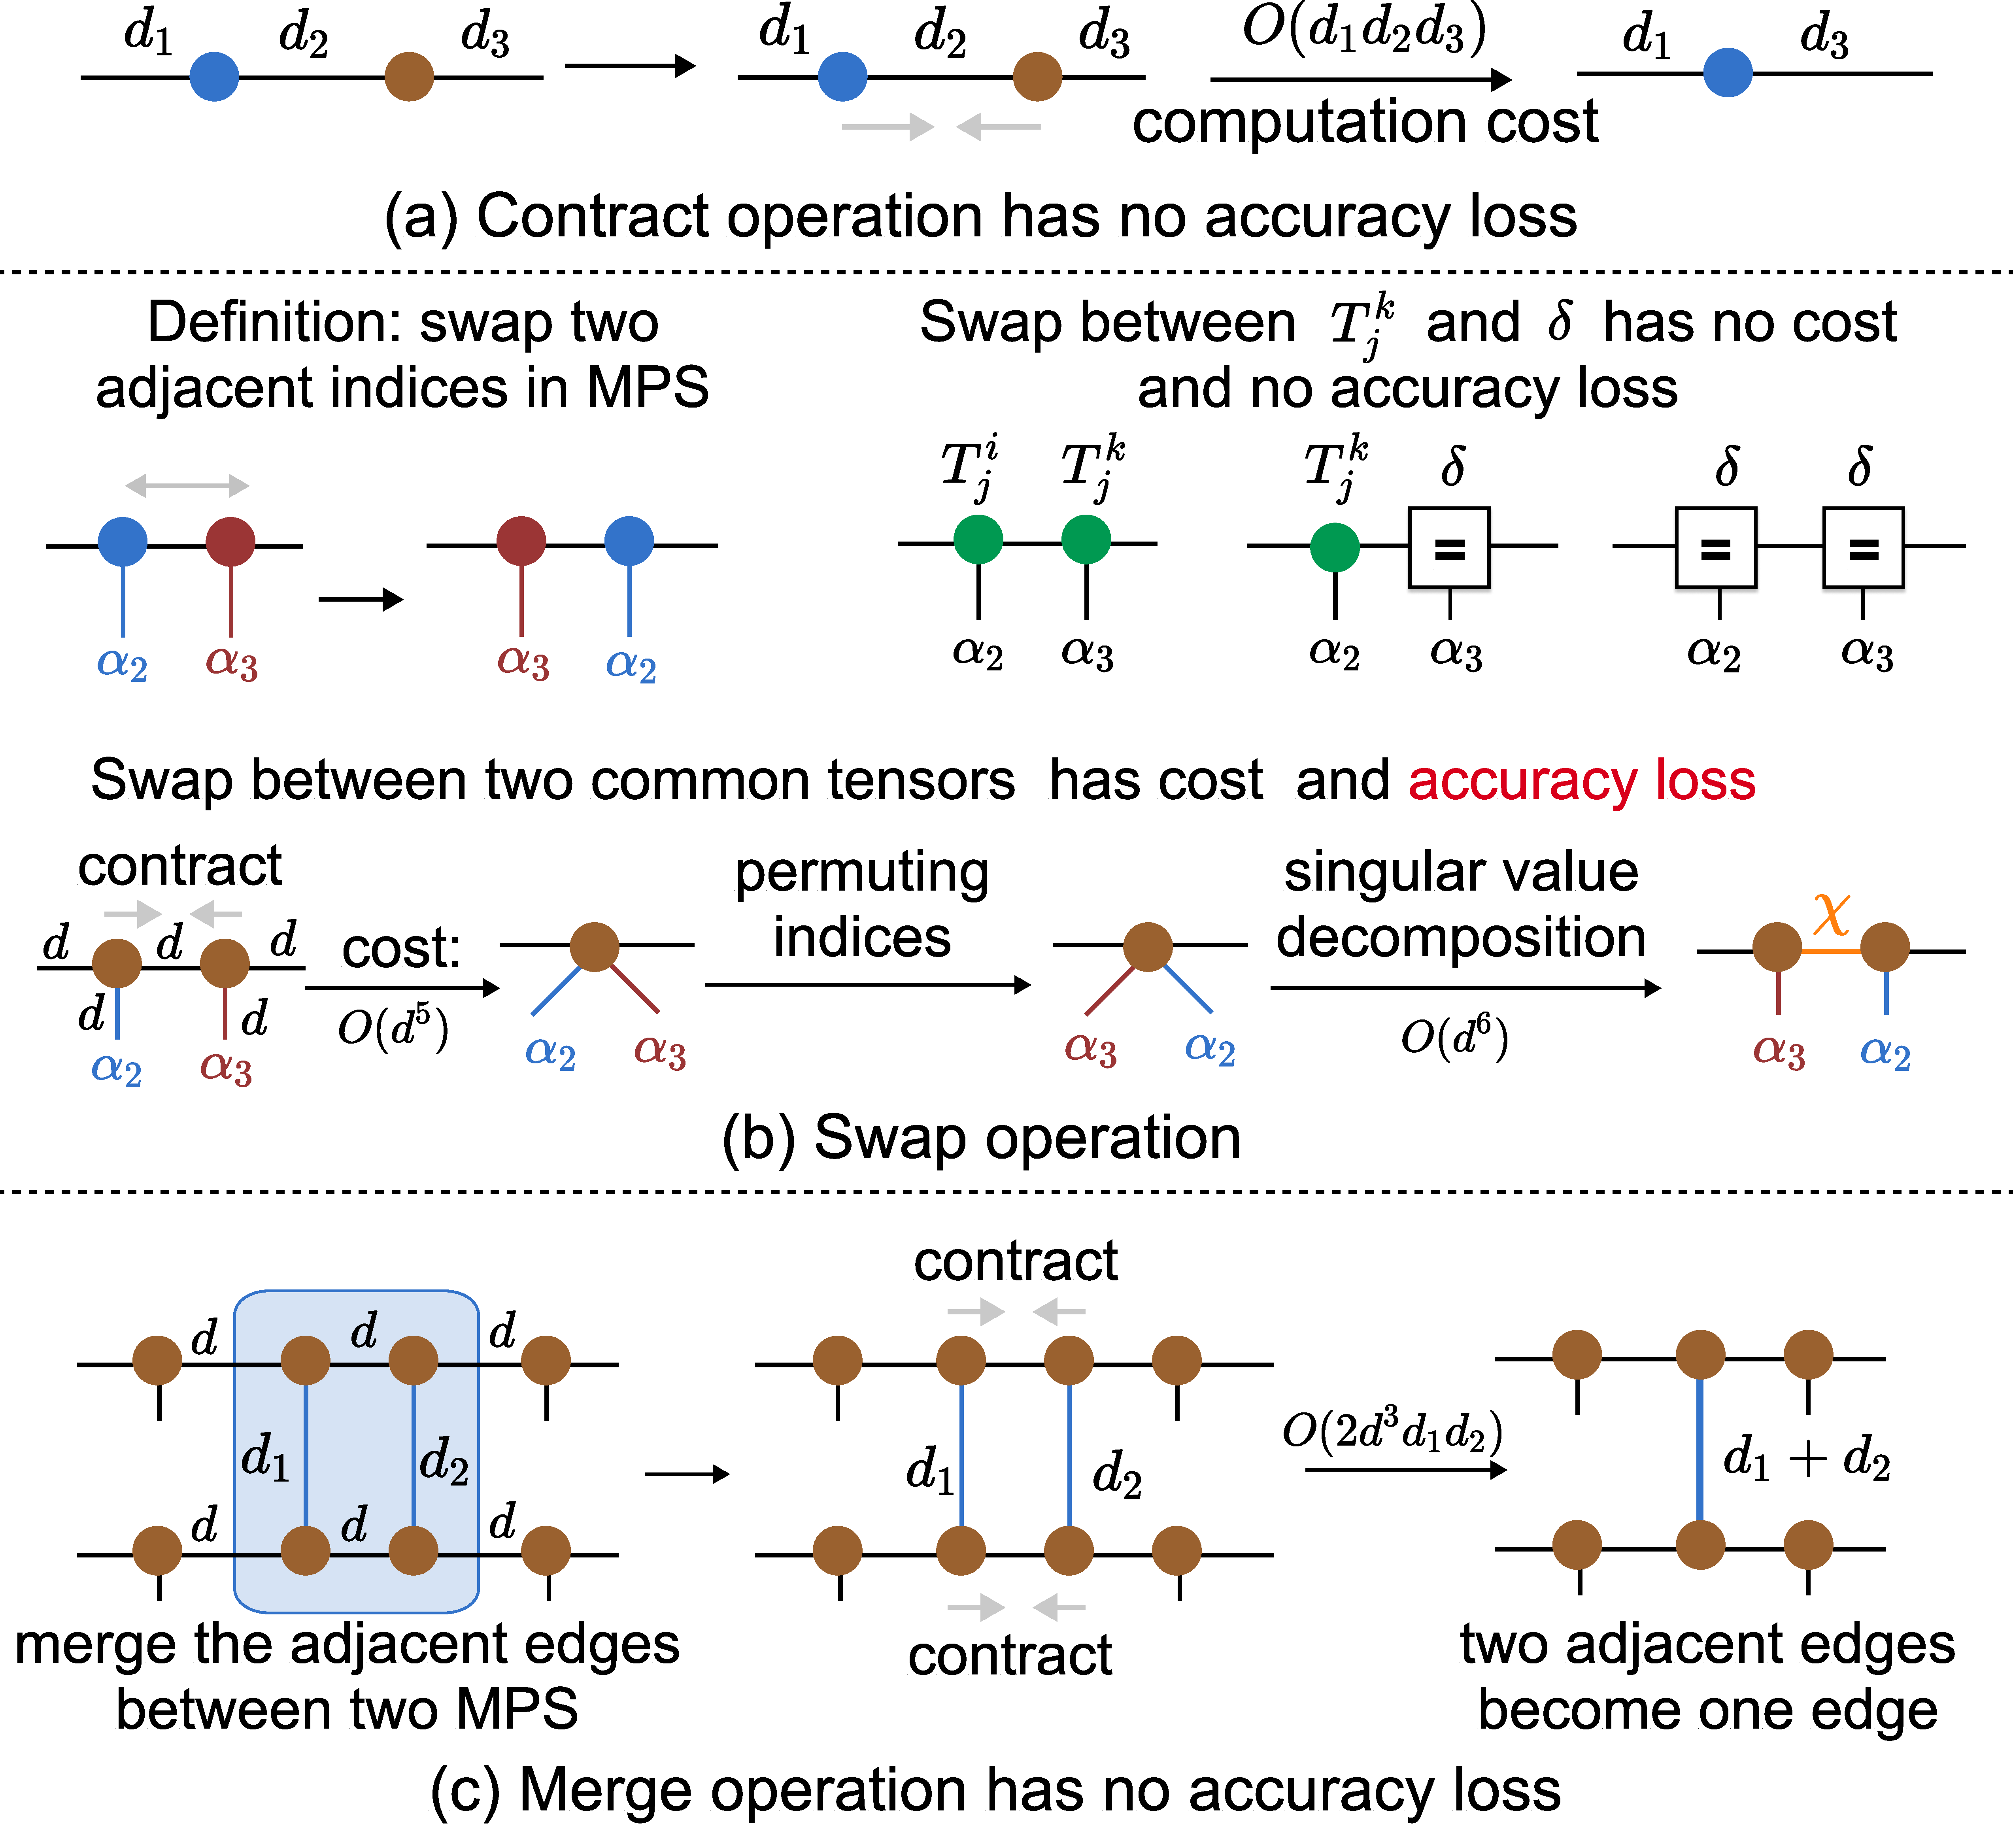
\includegraphics[width=1\columnwidth]{figures/operations.pdf}}
\vspace{-0.4cm}
\caption{Operations definition and cost in offline contraction.} 
\vspace{-0.4cm}
\label{fig:operations}
\end{figure}

\begin{algorithm}[t]
\small
\caption{Contraction-swap-merge Algorithm} \label{algo:contraction}
\KwIn{Tensor network with tensors \( A^{(1)}, \dots, A^{(n)} \), connectivity Tanner graph \( G(V, E) \), set of tensors with outer logical and syndrome indices \( P \subseteq V \)}
\KwOut{1D-chain MPS containing tensors in \(P \)}
Exactly decompose every tensor to MPS\label{line:decompose}\;
\While{\( \exists v \notin P \)}{\label{line:while}
    Find edge \( (i, j) \gets \arg\min_{(\mu, \nu) \in E, \{ \mu, \nu \} \not\subseteq P}  \) \( [ \sum_{b \in \partial \mu} \log(D_{b,\mu})  + \sum_{b \in \partial \nu} \log(D_{b,\nu}) - 2 \log(D_{\mu,\nu})] \) \label{line:argmin}\;
    Move tensor at edge \( (i, j) \) in \( A^{(i)} \) to MPS tail \label{line:move_tail}\;
    Move tensor at edge \( (i, j) \) in \( A^{(j)} \) to MPS head \label{line:move_head}\;
    \textit{Contract} edge \( (i, j) \) to combine MPS \( A^{(i)} \) and \( A^{(j)} \) into a new MPS\label{line:merge}\;
    Update \( E \gets E \setminus \{(i, j)\} \) \label{line:remove_edge}\;
    \For{\( k \in \partial j \)}{\label{line:for}
        Remove \( (j, k) \) from \( E \) \label{line:remove_jk}\;
        \eIf{\( k \in \partial i \)}{\label{line:if}
            \textit{Swap} to place duplicate edges \( (i, k) \) adjacent in \( A^{(i)} \) \label{line:swap}\;
            \textit{Merge} adjacent tensors, combining edges to increase \( D_{k,i} \) \label{line:merge_tensors}\;
        }{
            Add \( (i, k) \) to \( E \) \label{line:add_edge}\;
        }
    }
    \eIf{\( j \in P \)}{
        Add \( i \) to \( P \) \label{line:add_p}\;
    }{
        Update \( V \gets V \setminus \{j\} \) \label{line:remove_node}\;
    }
}
\Return the 1D-chain MPS\label{line:return}\;
\end{algorithm}


% trade-off, algorithm

As we can see, the \textit{swap} operation is an approximation operation with some accuracy loss. Thus, we propose a greedy algorithm to reduce the use of the \textit{swap} operations, as shown in Algorithm~\ref{algo:contraction}. We use a graph \( G(V, E) \) to denote this tensor network, the node \( V \) representing the tensors and edges \( E \) representing the connected indices between tensors $A^{(i)},A^{(j)}$ with a bond dimensions \( D_{i,j} \). The initial bond dimension is 2. Tensors with outer logical and syndrome indices in set \( P \) are preserved, forming a 1D matrix product state chain as output. 
% The edges are contracted iteratively based on minimal cost, preserving outer indices. Bond dimensions exceeding \( \hat{D} \) are truncated via SVD. The process stops when a 1D chain of tensors with outer indices remains, returned as \( Z \).
Specifically, we first decompose the tensors into MPS representation using the exact decomposition (Line \ref{line:decompose}). Then the algorithm loops until all nodes are in the preserved set  \( P \) (Line \ref{line:while}), stopping at a 1D chain. It selects the edge \( (i, j) \) with minimal contraction cost (Line \ref{line:argmin}), moves tensors in \( A^{(i)} \) to the tail (Line \ref{line:move_tail}) and in \( A^{(j)} \) to the head (Line \ref{line:move_head}), then merges them by contracting edge \( (i, j) \) (Line \ref{line:merge}). The edge is removed from \( E \) (Line \ref{line:remove_edge}). For each neighbor \( k \) of \( j \) (Line \ref{line:for}), edge \( (j, k) \) is removed (Line \ref{line:remove_jk}). If \( k \) connects to \( i \) (Line \ref{line:if}), duplicate edges \( (i, k) \) are swapped to be adjacent (Line \ref{line:swap}) and merged, increasing \( D_{k,i} \) (Line \ref{line:merge_tensors}). If \( k \) is not connected to \( i \), edge \( (i, k) \) is added to \( E \) (Line \ref{line:add_edge}). If \( j \in P \), \( i \) is added to \( P \) (Line \ref{line:add_p}); otherwise, \( j \) is removed from \( V \) (Line \ref{line:remove_node}). The final 1D MPS chain is returned (Line \ref{line:return}).

\begin{figure}[t]
\centerline{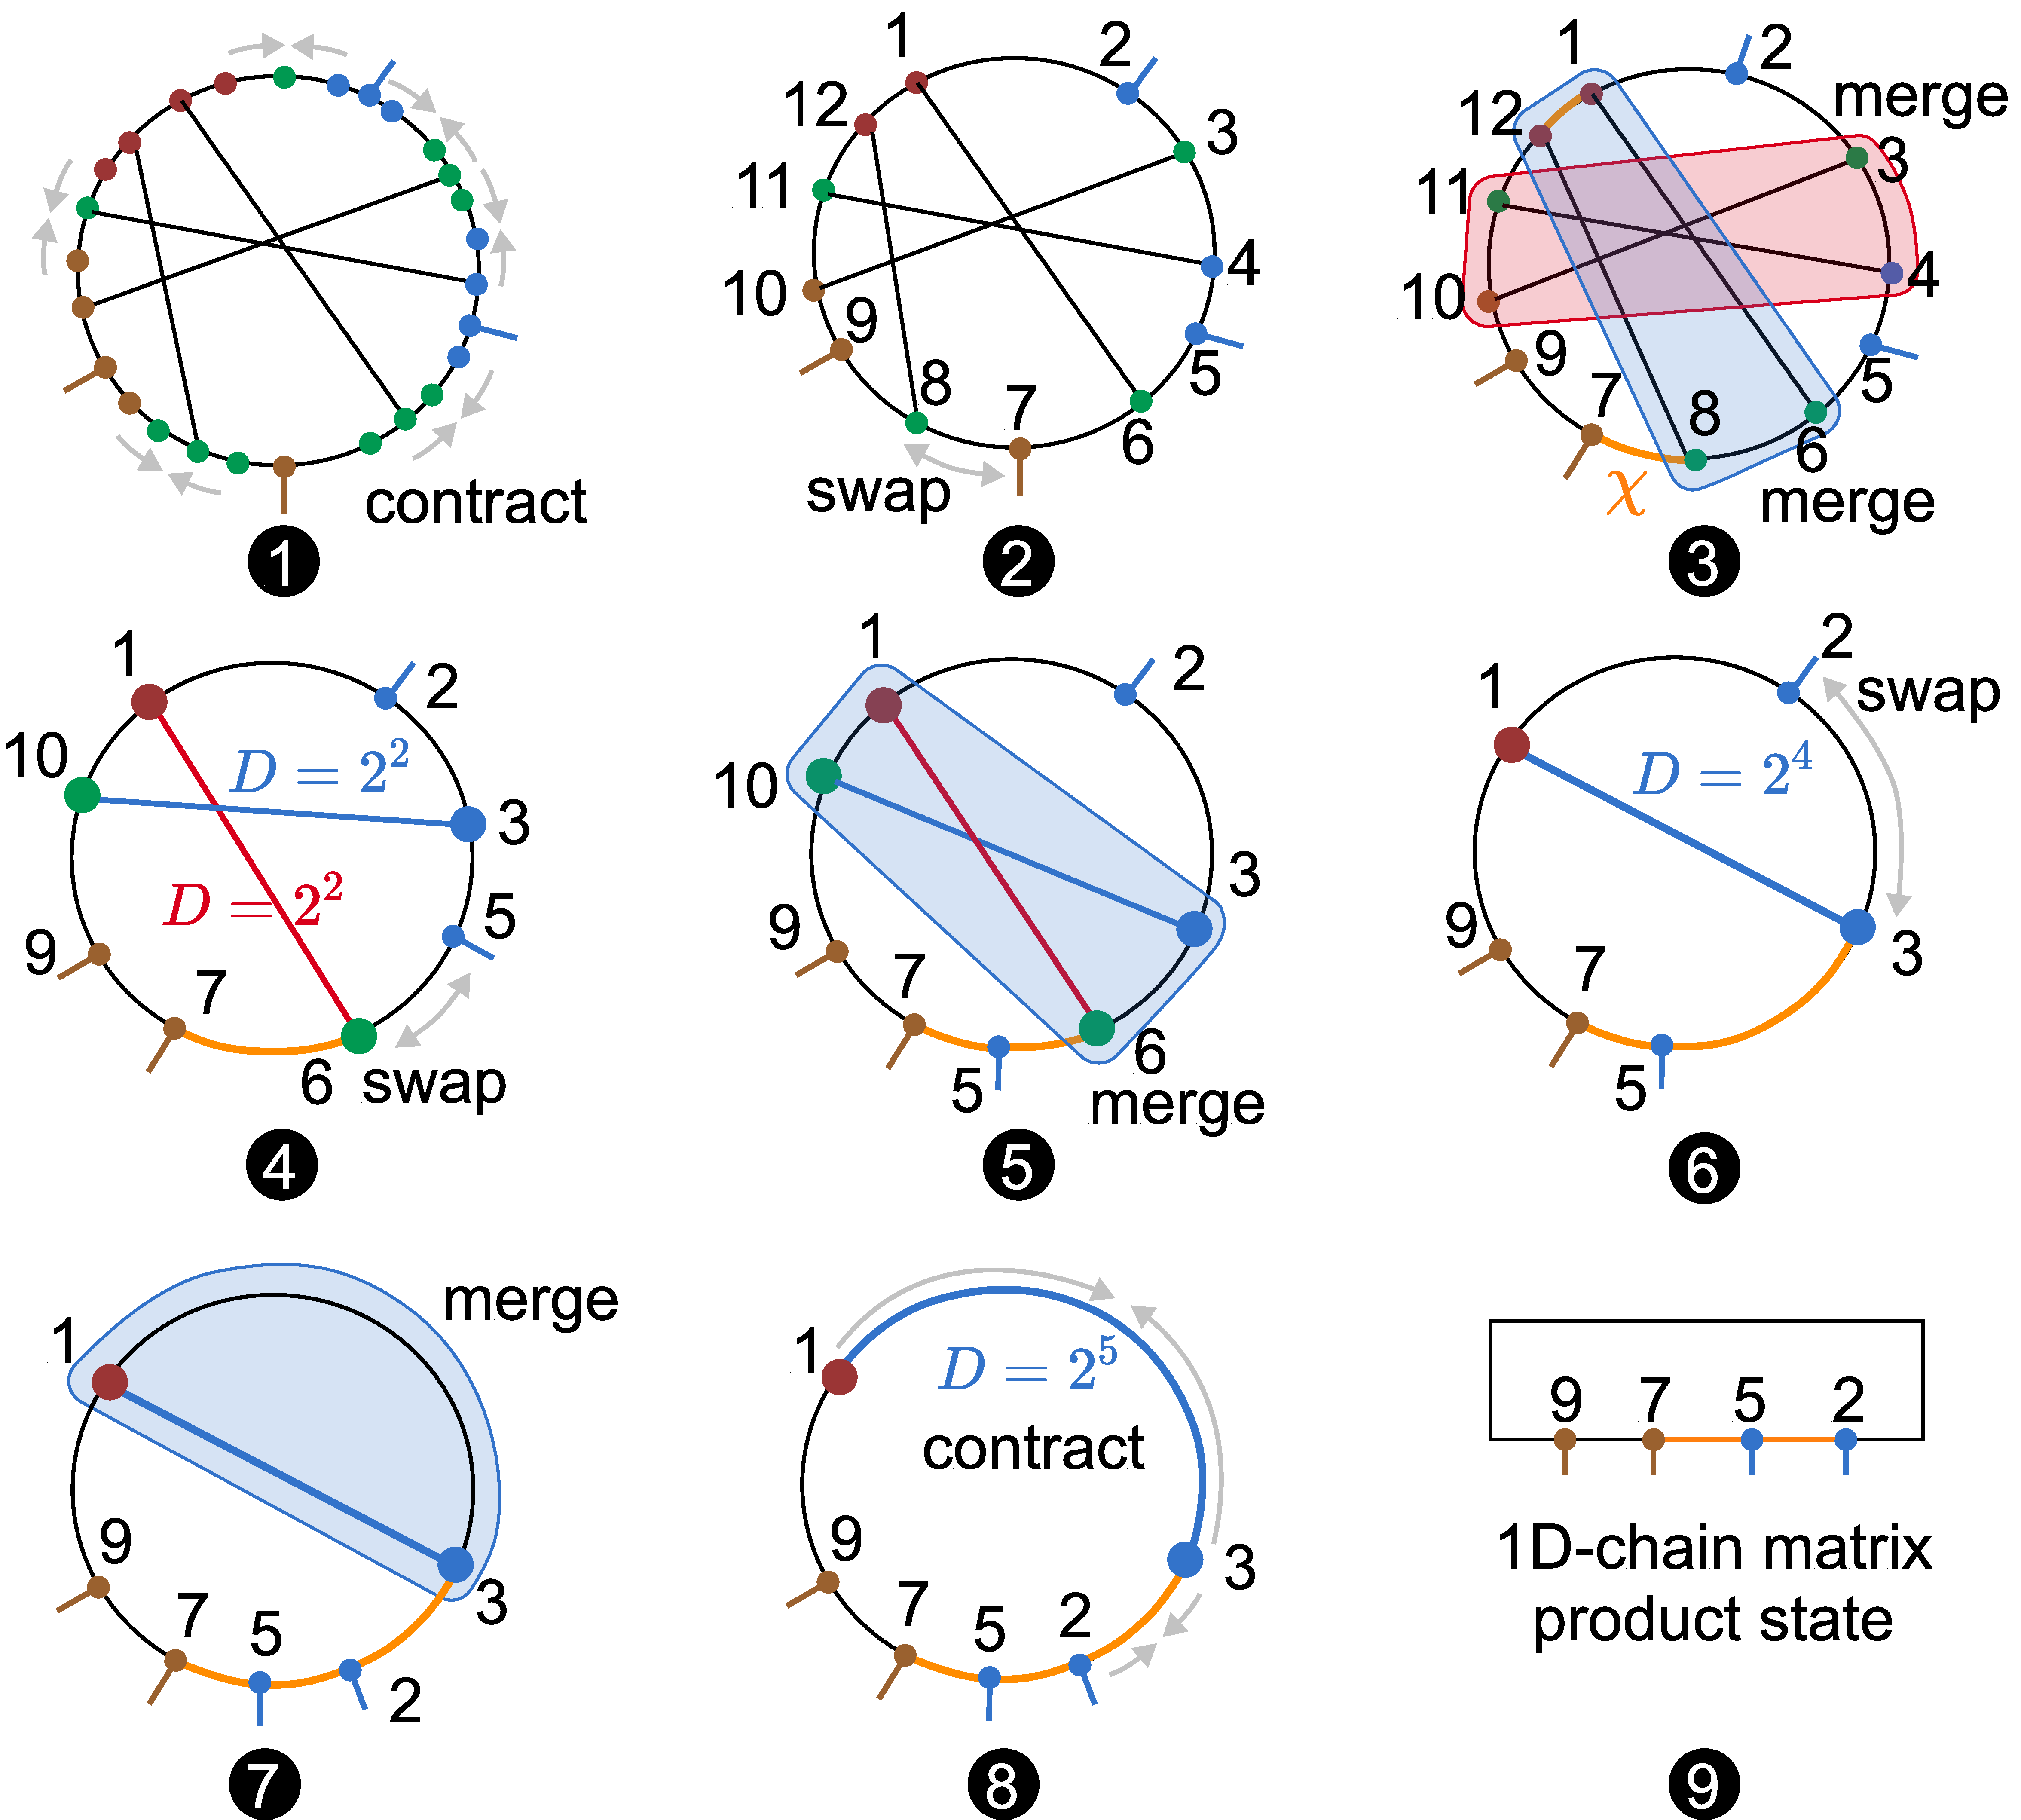
\includegraphics[width=0.9\columnwidth]{figures/circlecontraction9.pdf}}
\vspace{-0.2cm}
\caption{Offline contraction to get the approximated matrix product state for free energies under different syndromes.} 
% \vspace{-0.4cm}
\label{fig:contraction}
\end{figure}



\autoref{fig:contraction} gives an example of the \textit{swap-merge-contraction} approach. We start by \textit{contract} the edges in the MPS representation with the lowest contraction costs as shown in step~\ding{182}. Then we \textit{swap} the two MPS in edge (8,7) as step~\ding{183} to make the two pairs of edges (12,8) and (1,6) in adjacent positions as step~\ding{184}. We \textit{merge} the two pairs of edges \{(12,8) and (1,6), (11,4) and (10,3) \} into two new edges with the bond dimension $D=2^2$ as shown in step~\ding{185}. The steps \ding{185}-\ding{188} also repeat this \textit{swap} and \textit{merge} process until no edges are inside the circle. Then, we \textit{contract} the matrices (1,3) on the circle as in step~\ding{189}, except for the tensors \{9,7,5,2\} with outer logical and syndrome indices, to obtain a 1D-chain MPS with only logical and syndrome indices, as shown in step~\ding{190}.
